\section{Общая характеристика работы}
\textbf{Актуальность темы исследования.} Быстрые изменения происходящие в городской среде, как следствие 
технического прогресса требуют формирования новых методов в планирования инфраструктуры города для 
организации комфортной жизни людей. Это относится, в том числе, и к организации транспортной 
инфраструктуры, в частности к построению маршрутов общественного транспорта. Несмотря на кажущуюся 
хаотичность все перемещения пассажиров, подчиняются определенным закономерностям, связанным с масштабом и 
планировкой городской среды. Для принятия обоснованных решений по планированию или изменению маршрутной 
сети города необходимо выявить закономерности поведения населения и сформировать обобщенную модель, на 
основе которой можно строить и оценивать варианты транспортной системы. Для получения эффективных 
результатов, следует осуществлять принятие решений на основе актуальных данных, отражающих предпочтения 
жителей. В рамках магистерской диссертации следует разработать метод построения маршрутов общественного 
транспорта на основе предпочтений жителей.

\textbf{Цель и задачи работы.} данной работы являлось разработка метода генерации маршрутов общественного 
транспорта на основе предпочтений жителей для минимизации дискомфорта перемещения в городе. Для достижения 
поставленной цели решались следующие задачи:
\begin{itemize}
    \item генерация псевдореалистичных данных кластеров предпочтений;
    \item разработка методов маршрутизации между кластерами предпочтений;
    \item модификация и использование существующих алгоритмов для задачи маршрутизации;
    \item разработка критериев оценки качества построенных маршрутов;
    \item представление построенных маршрутов на карте;
\end{itemize}

\textbf{Объектом исследования} является построения маршрутов общественного транспорта на основе актуальных 
данных о предпочтениях жителей по перемещениям в современной городской среде. 

\textbf{Предметом исследования} является разработка и применение методов методы построения маршрутов 
общественного транспорта учитывающие актуальные данные о предпочтениях жителей по перемещению и 
интенсивности пассажиропотоков в городе.

\textbf{Гипотеза исследования.} Существующие системы используемые для анализа и построения маршрутных сетей 
городского транспорта не учитывают данные о предпочтении жителей по перемещении, что приводит к отрицательному 
влиянию на городской транспорт со стороны частного, а также к возрастанию загруженности дорожных сетей.

\textbf{Научная новизна} диссертационной работы заключается в:
\begin{itemize}
    \item Автоматизации процесса построения начальной маршрутной сети без участия транспортного инженера.
    \item Использовании разработанной методика построения сети маршрутов основанный на использовании данных о 
        предпочтении жителей.
    \item Предложении по модификации существующих алгоритмов для построение маршрутных сетей.
    \item Разработке нового алгоритм для построения сети маршрутов.
\end{itemize}

\textbf{Практическая ценность.}
В настоящее время построение или изменение маршрутов общественного транспорта происходит при участии 
транспортного инженера, которому необходимо вручную предлагать варианты по изменению, а система проводит 
работу только по оценке предложенного маршрута. 

Данная разработка может быть использована для:
\begin{itemize}
    \item автоматизации процесса построения начальной маршрутной сети или отдельных маршрутов;
    \item модификации существующей маршрутной сети или отдельного маршрута с использовании данных о 
        предпочтении;
    \item комплексного анализа построенной сети или маршрута с использованием данных о предпочтении, длине 
        построенной сети и т.п.;
\end{itemize}

\textbf{Публикации.} По материалам диссертации автором опубликовано 3 работы, 2 из которых представлены 
в рецензируемом научном журнале, входящем в перечень Высшей аттестационной комиссии. 

\textbf{Структура и объём работы.} Диссертационная работа состоит из введения, четырех глав, заключения, 
списка использованных источников из 60 наименований и насчитывает 93 страници, в том числе 60
страници основного текста, 20 рисунков, 1 таблицу и 3 приложения.

\section{Основное содержание работы}
\textbf{Во введении} обосновываются выбор темы диссертационного исследования и ее актуальность, определяются 
цели и задачи работы, объект, предмет и гипотеза исследования, формулируется научная новизна.

\textbf{В первой главе} приводятся результаты исследования предметной области. Произведён анализ общего 
состояние существующей проблемы в транспортной инфраструктуре. Описаны существующие программные продукты 
частично решающие данную проблему в полуавтоматическом режиме, но требующие вмешательства транспортного 
инженера для проектирования транспортной сети. Также рассмотрена литература по современным исследованиям в 
данной области и методам предлагаемых в них. В результате сформирован подход органично вписывающийся в 
существующую систему построения для решения поставленной задачи.

Следует отметить, что развитие транспортной инфраструктуры основывается на устаревших нормативах, не 
учитывающих стремительное увеличение личного транспорта и изменений функционального назначения городских 
пространств. Это ведет к ухудшению транспортной ситуации, снижению качества транспортного обслуживания, 
увеличению пробок, и как следствие к усилению неудовлетворенности жителей. Критичным фактором является 
игнорирование фактических предпочтений жителей по перемещению по городу при проектировании маршрутов 
городского транспорта.

Для оптимизации маршрутной сети общественного транспорта необходимо проанализировать большой объем данных, 
характеризующих численность и мобильность населения, среднее время перемещения, расположение мест приложения 
труда и жилых массивов. Источниками этих данных выступают статистические сборники, выписки о численности 
сотрудников крупных предприятий, собираемые муниципальными предприятиями общественного транспорта, 
информация о количестве проданных билетах на маршрутах общественного транспорта. Для сбора данных о 
перемещениях жителей организуется целый комплекс мероприятий по натурному подсчету пассажиропотока в 
подвижном составе общественного транспорта и на остановочных пунктах существующих маршрутов, а также 
анкетированию жителей. Такие традиционные методы являются достаточно трудоемкими, а полученные данные не в 
полной мере отражают динамично меняющуюся ситуацию. В связи с этим, необходимо использовать современные 
технологии и новые ресурсы для получения актуальных данных о предпочтениях жителей по перемещениям в городе 
и интенсивности пассажиропотоков. Основываясь на современных подходах к анализу данных можно получить 
ценную информацию для поддержки принятия решений в процессе планирования развития транспортной системы 
города.

\textbf{Во второй главе} рассмотрены и проанализированы существующие методы применимые к задаче формирования 
маршрутов, а также разработаны методы на их основе для формирования маршрутных сетей используя 
кластеризованные данные о предпочтения по перемещению в городе.

Сформулируем постановку задачи формирования маршрутов. Пусть заданы \( n_s \)~-- число узлов (остановочных 
пунктов), \( n_r \)~-- число маршрутов. Требуется построить \( n_r \) последовательностей узлов, при которых 
целевая функция качества маршрутной сети будет принимать максимальное значение. 

Задача тесно связана с задачей маршрутизацией <<из пункта А в пункт Б>>, но имеет некоторые отличия. 
Во-первых, в типовой задаче маршрутизации целевая функция – это время поездки от начала до конца маршрута, 
которое необходимо минимизировать. В случае с построением сети маршрутов общественного транспорта целевая 
функция -- интегральная, учитывающая средние показатели времени пешего хода до остановки, длины пути, 
количества пересадок, и пр. Во-вторых, в типовой задаче маршрутизации для движения выбираются любые 
промежуточные точки, сокращающие маршрут, тогда как в рассматриваемой задаче промежуточные точки 
расположены там же, где и центры кластеров.

Для формирование начальной сети маршрутов был разработан метод использующий принцип <<минимального>> 
увеличения длины маршрута при включении нового пункта, принцип работы которого заключается в итеративном 
добавлении в существующие маршруты узлы, минимально увеличивающие длину исходных маршрутов. Псевдокод 
представлен алгоритмом \ref{alg:min-length}.

На вход алгоритма подаются: \( n_r \) -- число маршрутов в сети, \( n_c \) –- число узлов (центров 
кластеров), \( C_t \) – множество терминальных узлов (определенных посредством построения окружности, 
содержащей все узлы), \( C_{nt} \) -- множество нетерминальных узлов (сумма элементов множества терминальных 
и нетерминальных узлов равна числу центров кластера), матрица длин размером 
\( ||{C_{nt}} + {C_{t}}|| \times ||{C_{nt}} + {C_{t}}|| \). Заметим, что \( C_t + C_{nt} = n_c \)

Выходом алгоритма является транспортная сеть \( R_i \), содержащие непересекающиеся множество узлов, 
\( r_{i} = [p_{1}^{(i)}, \dots, p_{k}^{(i)}] \), где \( i = 1, \dots, n_r \). 

В результате работы алгоритма получаем результат, в зависимости от используемой стратегии, представленный на 
рисунках \ref{fig:graph} и \ref{fig:osrm}
\begin{figure}[ht!]
    \centering
    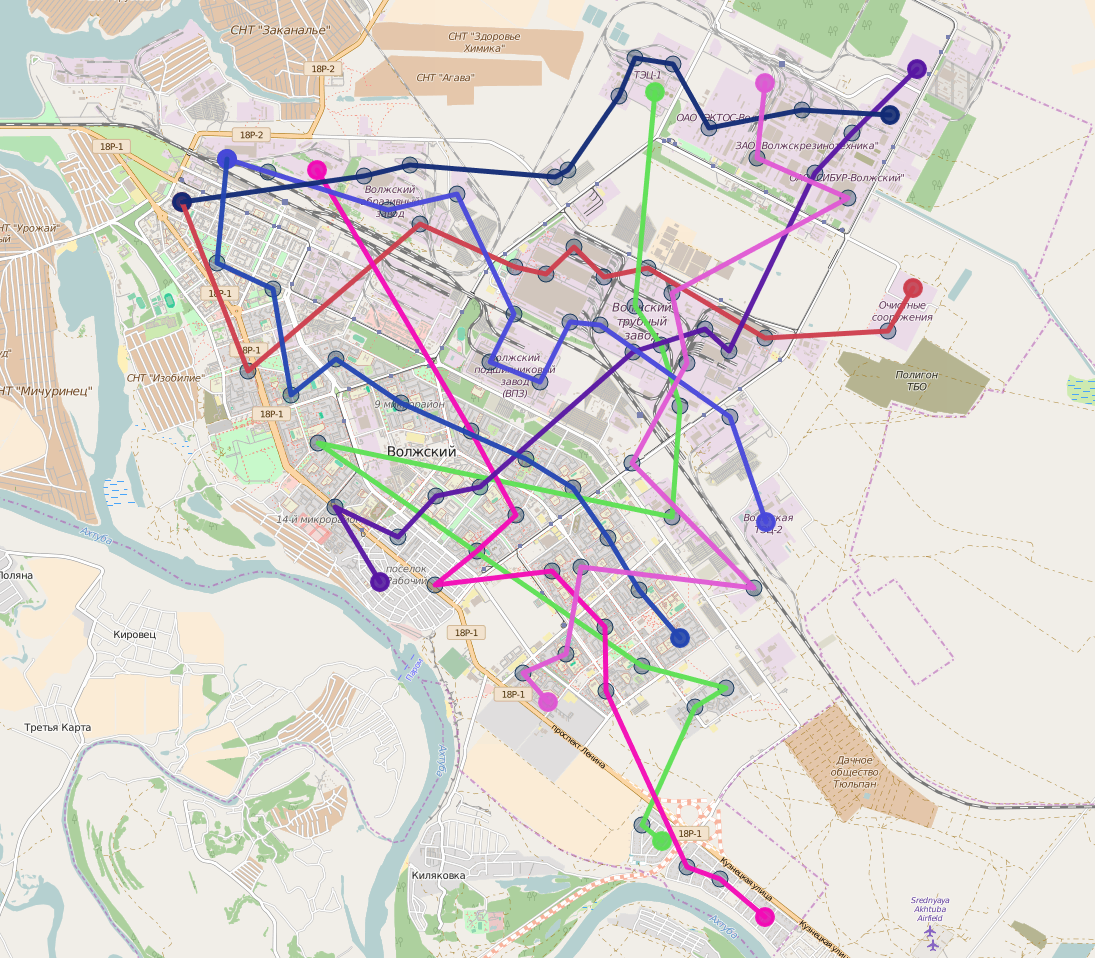
\includegraphics[width=0.75\textwidth]{100-8}
    \caption{Построением маршрута по графу (страгегия 'graph')}
    \label{fig:graph}
\end{figure}

\begin{figure}[ht!]
    \centering
    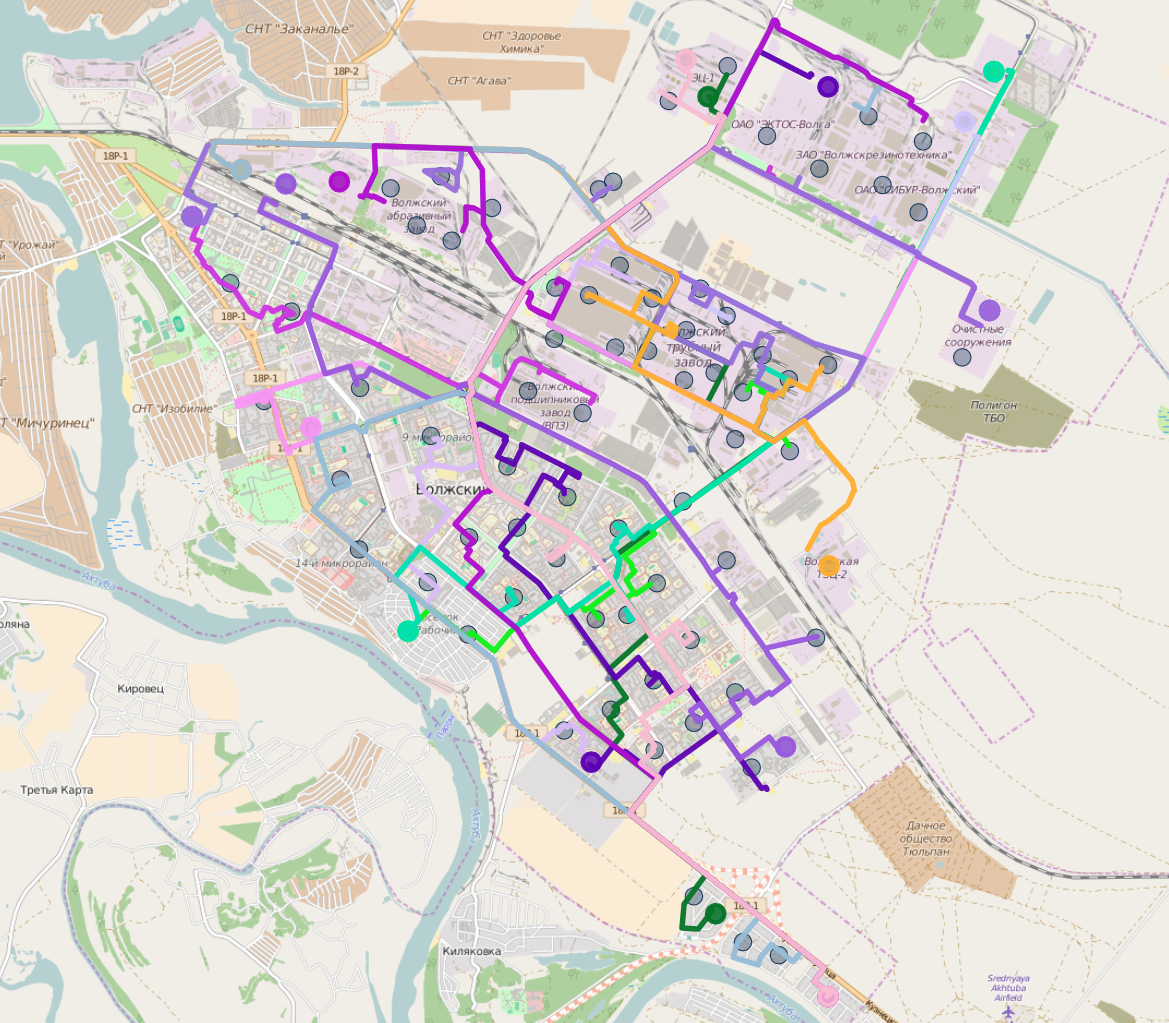
\includegraphics[width=0.75\textwidth]{100-14}
    \caption{Построением маршрута по дорогам (стратегия 'OSRM')}
    \label{fig:osrm}
\end{figure}

\begin{algorithm}[ht!]
    \caption{Алгоритм построения маршрутной сети}
    \KwData{\( n_r, C_t, C_{nt} \)}
    \KwResult{\( R_i \) -- список маршрутов сети.}
    1. Создать сеть \( R_i \) соединяющий вершины \( C_t \)\;
    2. \ForEach{\( i \)-го маршрута из сети \( R_i \)}{
        1. Поместить вершины маршрута (попарно) в список \( PN \)\;
        2. Найти вершину \( c_j \) (из \( C_{nt} \)), присоединение которой минимально увеличивает 
            длину маршрута из \( PN \) и добавить новый маршрут в список \( RC \)\;
        3. Составить новый список \( RCC \) состоящий из маршрутов, полученных путём замены пар 
            вершин \( PN \) на изменённые \( RC \)\;
        4. Рассчитать длины маршрутов в списке RCC, используя OSRM\;
        5. Выбрать из \( RCC \) маршрут \( R^{\star}_i \) с минимальной длиной\;
        6. Заменить \( R_i \) на \( R^{\star}_i \)\;
        7. Удалить узел \( c_j \) из \( C_{nt} \) добавленный в \( R^{\star}_i \)\;
    }
    3. Если список \( C_{nt} \) не пустой, перейти на шаг 2, иначе закончить построение\;
    \label{alg:min-length}
\end{algorithm}

\clearpage

\textbf{В третье главе} описана методология проектирования ПО, разработана методика проведения эксперимента, 
произведено испытание разработанных алгоритмов, а также обсуждены полученные результаты в ходе эксперимента 
и сделан вывод на их основе. Предложенные алгоритмы были реализованы с использованием языка программирования 
Python и сервиса построения маршрутов Open Source Routing Machine (OSRM) для расчёта расстояния между узлами 
графа по городским дорогам.

Для работы были сгенерированы данных о предпочтениях по перемещению жителей среднего по размерам города с 
примерным числом жителей около \( 350\ 000 \). В качестве результата, было получено \( 6000 \) пар точек 
отправления-назначения или \( 12000 \) точек в общей сложности. Для того чтобы понять какое количество 
кластеров (или узлов) влияет на эффективность работы предложенного алгоритма было предложено произвести 
варьирование параметров: количество кластеров и количество маршрутов для построения.

\textbf{В четвёртой главе} произведена оценка эффективности разработанных алгоритмов. Для оценки 
эффективности алгоритма и изучения его специфики, были проведены эксперименты в ходе которых менялось 
количество узлов в дорожном графе и количество создаваемых маршрутов в городской сети, а также несколько 
вариантов реализации данного метода. Наиболее интересным случаем является, когда обрабатывается большое число 
узлов в графе или большое число геопространственных данных.

Чтобы понять эффективность работы алгоритма в зависимости от окружающей среды, были разработаны три 
альтернативных реализации:
\begin{enumerate}
    \item Последовательная реализация (или 'graph') алгоритма основанного на графе дорог. В данной реализации 
        предполагается, что связь между узлами может быть проведена по прямой линии, несмотря на состояние 
        дорог. Эту реализацию можно рассматривать в качестве базовой.
    \item Последовательная реализация с использованием OSRM (или 'S.OSRM') -- это усовершенствованная версия 
        предыдущей стратегии, где расстояние между кластерами рассчитывается с использование движка 
        маршрутизации OSRM по дорожной сети.
    \item Параллельная версия с использованием OSRM (или 'P.OSRM') предполагает возможность в 
        распараллеливании внутреннего цикла алгоритма.  
\end{enumerate}

В результате работы получены следующие данные представленные на рисунках \ref{fig:result-01} и 
\ref{fig:result-02}
\begin{figure}[ht!]
    \centering
    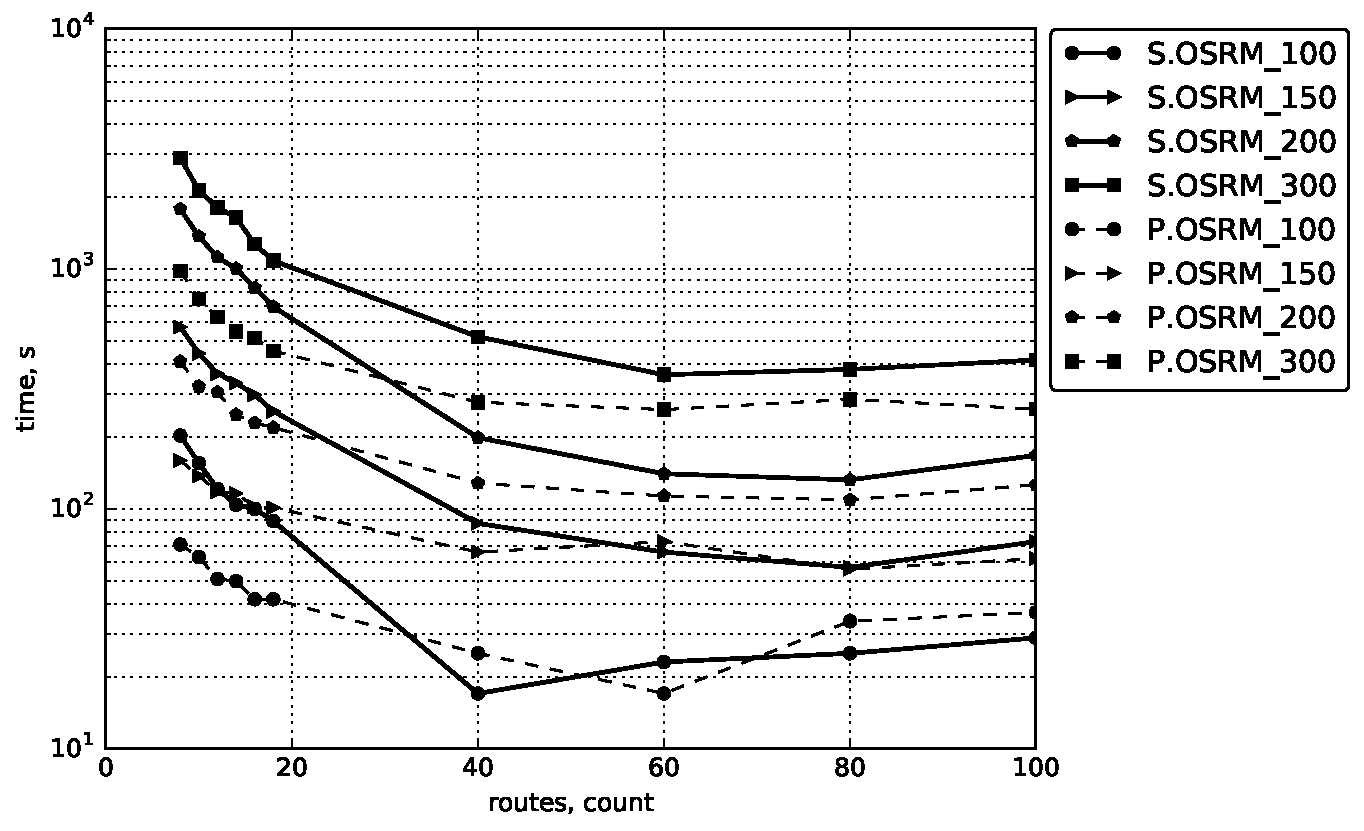
\includegraphics[width=\textwidth]{result-01}
    \caption{Зависимость времени построения от количества маршрутов}
    \label{fig:result-01}
\end{figure}

\clearpage

\begin{figure}[ht!]
    \centering
    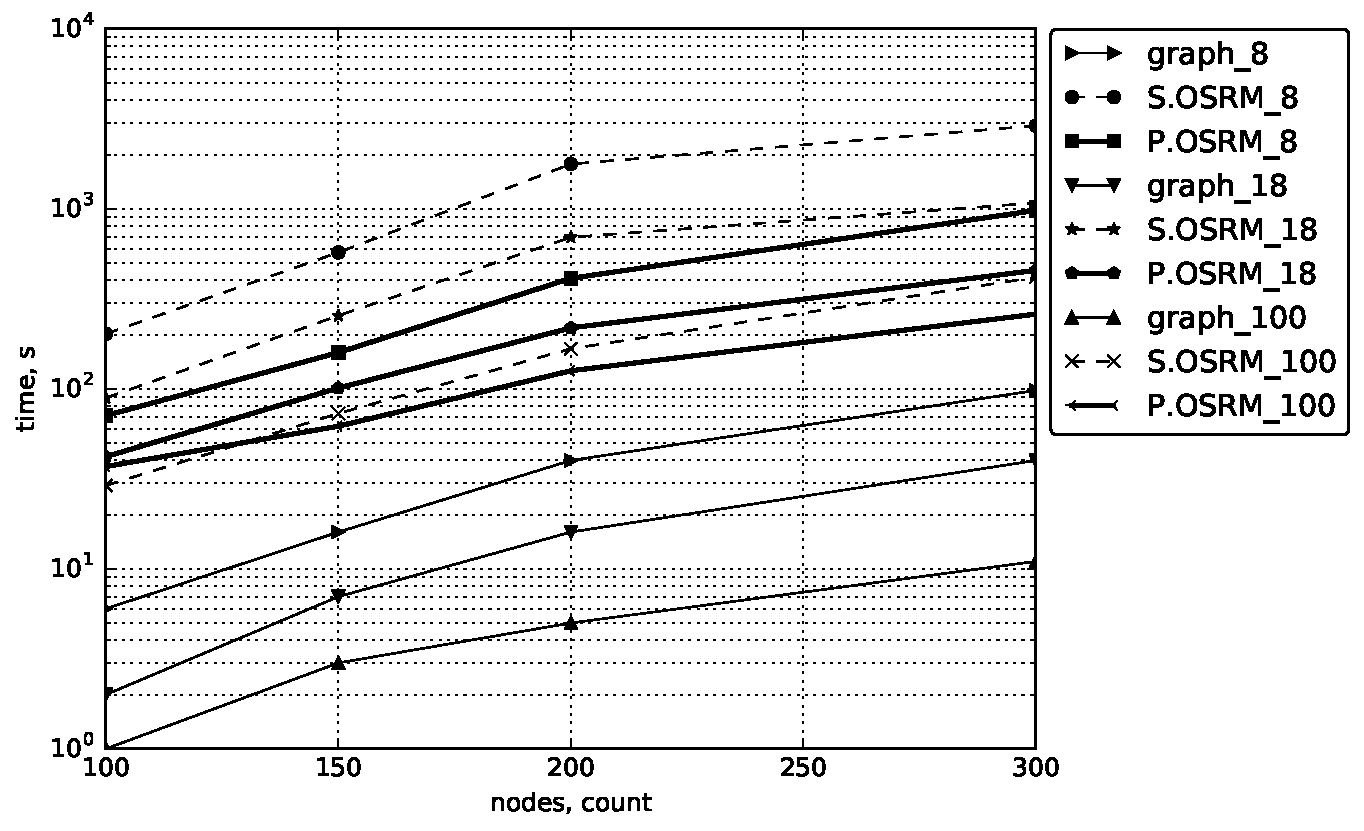
\includegraphics[width=\textwidth]{result-02}
    \caption{Зависимость времени построения от количества кластеров}
    \label{fig:result-02}
\end{figure}

\textbf{В заключении} работы сформулированы общие выводы по проделанной работе в рамках магистерской 
диссертации, обсуждены полученные результаты по разработанному алгоритму, произведена эмпирическая оценка 
сложности, а также выделены его сильные и слабые стороны.

\textbf{В приложении} приведены материалы справочного, иллюстративного характера и техническое задание на 
создание программы формирования маршрутов общественного транспорта на основании обработки данных.

\section{Основные результаты работы}
\begin{itemize}
    \item Рассмотрены системы используемые для анализа транспортной сети;
    \item Изучены алгоритмы используемые для задачи построения маршрута;
    \item Предложен алгоритм формирования маршрутной сети на основе обработки данных о предпочтении;
    \item Реализован алгоритм формирования маршрутной сети на основе обработки данных о предпочтении;
    \item Проверена эффективность трёх стратегий реализованного алгоритма на сгенерированном наборе данных;
\end{itemize}

\section{Перспективные направления развития работы}
Согласно результатам полученным в работе предложенный алгоритм может быть использован для создания 
предварительной сети маршрутов общественного транспорта. Также разработанный модуль может быть использован 
как компоненты системы для создания начальной сети с последующей её модификацией.

\renewcommand{\bibname}{Публикации по теме диссертации}
\begin{thebibliography}{10}
    \bibitem{first} Strategway: web solutions for building public transportation routes using big geodata 
        analysis / Golubev A., Chechetkin I., Solnushkin K.S., Sadovnikova N., Parygin D., Shcherbakov M., 
        Brebels A. // Proceedings of The 17th International Conference on Information Integration and 
        Web-based Applications \& Services (iiWAS2015) (December 11 - 13, 2015 Brussels, Belgium) 
        ACM New York, New York pp. 665 - 668
    \bibitem{second} Комплекс инструментов интеллектуального анализа данных strategway для поддержки 
        принятия решений по управлению развитием инфраструктуры города / Садовникова Н.П., Щербаков М.В., 
        Парыгин Д.С., Солнушкин К.С., Голубев А.В., Чечёткин И.А. // В сборнике: Развитие средних 
        городов: замысел, модели, практика Материалы III Международной научно-практической конференции. 
        Волгоград, 2015. С. 147-150
    \bibitem{third} Автоматизация поддержки принятия решений по разработке маршрутов общественного 
        транспорта на основе анализа данных о корреспонденциях жителей / М. В. Щербаков, 
        Н. П. Садовникова, Д. С. Парыгин, А. В. Голубев, И. А. Чечеткин // Вестник компьютерных и 
        информационных технологий. -- М. : Издательский дом <<Спектр>>, 2016. -- Принята к печати.
    \bibitem{fourth} Maxim Shcherbakov and Alexey Golubev, An algorithm for initial public transport network 
        design over geospatial data // 2016 IEEE International Smart Cities Conference (ISC2) (ISC2 2016) 
        (September, 2016 Trento, Italy)
\end{thebibliography}